\section{Auto-encoder Network Evaluation}
\label{exp}

In this section, we firstly briefly review the auto-encoder network model constructed with theta neurons
proposed in the paper, and then describe how we reproduce the results of the experiments conducted by the author.

\begin{figure}
\centering
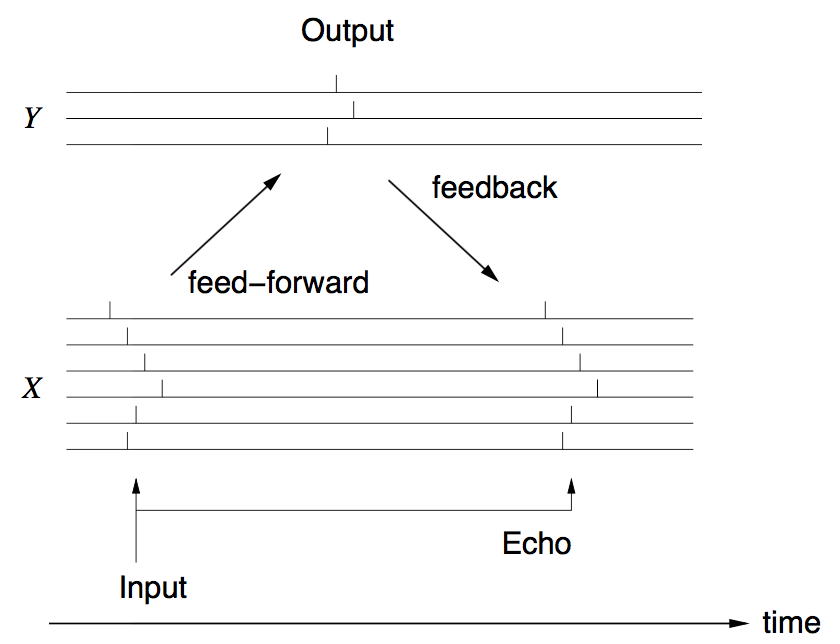
\includegraphics[width=0.98\columnwidth]{network}
\caption{The auto-encoder network tries to reconstruct the input spikes at target firing times (the echo of the input burst).
}
\label{auto_encoder}
\end{figure}

In the original paper, the author explains how to train a network to predict its own activities using the learning rule derived above. 
The prediction objective is a time-delayed version of the input (echo), 
and the network has to find a representation of the input that minimizes mean squared reconstruction error.
Figure~\ref{auto_encoder} shows the simplified architecture of the auto-encoder network.
The network consists of three layers of neurons: 
an input population $X$ of size $n$ neurons represents the input vectors using spike times; 
an output population $Y$ of size $m$ neurons is activated by neurons in $X$; 
a reconstruction population $X'$ of size $n$ neurons is activated by neurons in $Y$ and reconstructs the input (with a predefined delay).

Usually $m < n$, so what the auto-encoder network does is to learn a compact representation of the input data,
and reconstruct the input from the representation. 
We can also view the process as reducing the dimension (compressing) of the original input data,
and then reconstructing them.
We hope to find a good representation so that the reconstruction error (the difference between the reconstructed
data and the original data) is as little as possible.

The author proposes in the paper that if the spike times are within the linear part of the response curve,
then the auto-encoder network performs Principal Component Analysis (PCA) in the time domain.
And in the experiment section of the paper, the author shows how to train an auto-encoder network to compute PCA
of a two-dimensional Gaussian distribution.
We redid all the experiments mentioned in the paper. 
In the following subsection, 
we describe our experiment results and focus on comparing the results obtained by the author and us.

\subsection{PCA of a Gaussian Distribution}

In this experiment, we use three input neurons to encode a two-dimensional Gaussian random variable.
Specifically, the spike times of the three neurons (denoted by $t_0$, $t_1$, and $t_2$) encode the two 
dimensions of the Gaussian random variable by the two relative spike times $t_1 - t_0$ and $t_2 - t_0$, 
where the spike time of the first neuron $t_0$ is used as an absolute time reference.

We construct the 3-2-3 network ($n=3$, $m=2$) and set the parameters such as $ISI$ and $C$ to the same
value described in the paper.
We randomly generate 500 input sample points and use them to train the auto-encoder network.
The evolution of the six weights over iterations are shown in Figure~\ref{local_minimum}.
We can see that the weight converges to a stable solution, and the MSE significantly decreases.
However, the learned weight matrix is only a local optimal solution, as the reconstructed $t_i$s for each input sample
always satisfy that $t_0 \approx t_1 \approx t_2$. 
That's why in Figure~\ref{local_minimum}(c) we see that the reconstructed relative spike time is always $0$,
no matter what the $\bar t_i$s (the desired spike times) are.
Note that the author didn't mention the problem of local minimum, 
neither did he explain why in Figure 5 of the original paper, the weights converge to a value near
1.5 in the beginning but diverge after several hundred of iterations even though the learning rate $\eta$
is only 0.0001 as provided in the paper.

To get out of the local minimum, we have to increase the learning rate $\eta$. 
Practically, we change $\eta$ to nearly $0.1$ and continue training starting from the weights of 
the local minimum solution. The results are shown in Figure~\ref{local_better}.
We can see that the weights diverge at first, and then become stable or oscillate around some fixed values,
and the MSE decreases to a lower level.

However, the weight matrix is still local optimal, 
as we can see in Figure~\ref{local_better} the reconstruction error of points
satisfying $t_1 < t_0$ and $t_2 < t_0$ (``negative samples'') is relatively large. 
In other words, the auto-encoder network successfully learns one direction of the principal component but fails
to learn the other one. To solve the problem, we dynamically set a higher learning rate $\eta$ when
the model is fed with samples where $t_1 < t_0$ and $t_2 < t_0$ and a lower learning rate otherwise,
which is equivalent to resampling the negative samples.
In this way, we get results shown in Figure~\ref{global_best}.
Some of the weights oscillate again, and then all weights become stable (see Figure~\ref{global_best}(a)).
The MSE further decreases (see Figure~\ref{global_best}(b)).
The shape of the reconstructed principal directions is exactly the same with that shown in the paper.
We finally reproduce the PCA results successfully.

The reason why the author could train the model to do PCA without dynamically tuning the learning rate is not yet known.
All experiments we conducted using the exactly same parameters as the author showed in the paper failed to reconstruct the principal directions as the weight matrix always ended up in a local optimal solution.
We discuss this mismatch more in Section~\ref{discussion}.

\begin{figure*}
\centering
\subfigure[$w_i$s]{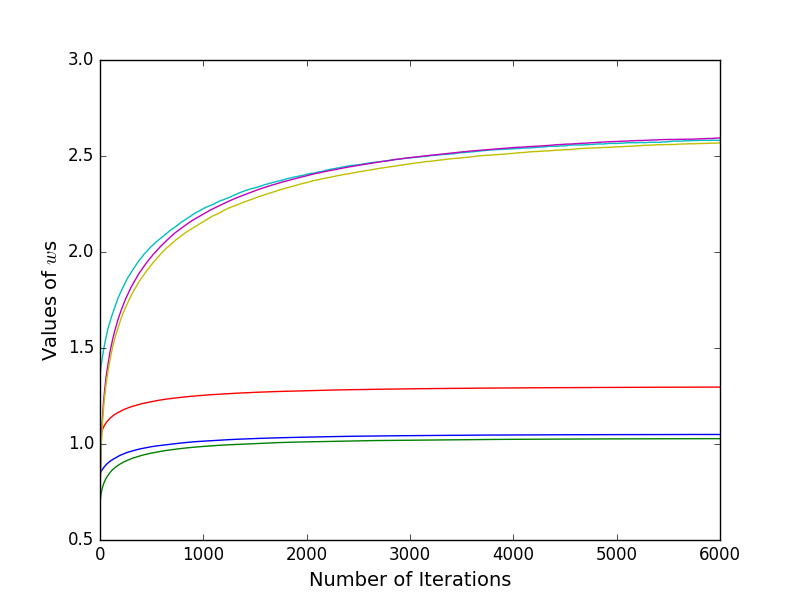
\includegraphics[width=0.68\columnwidth]{local_min_weight_evolution}}
\subfigure[MSE]{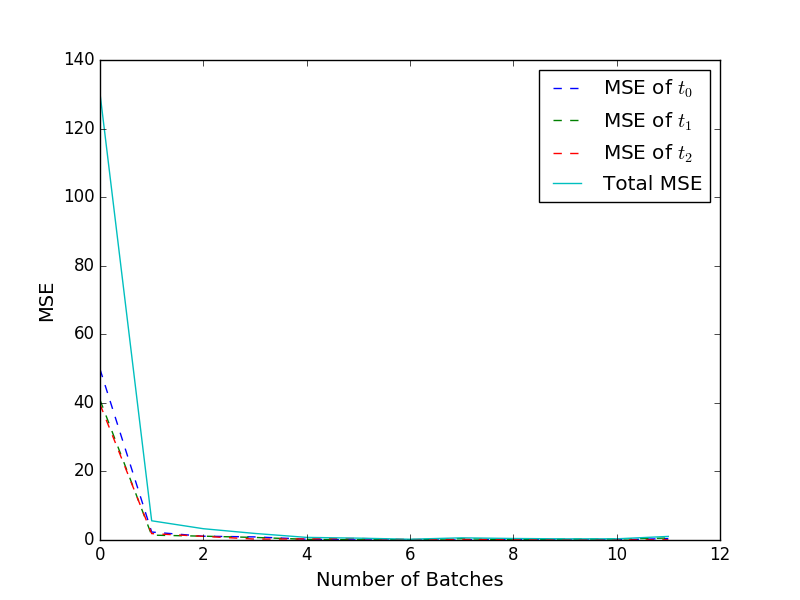
\includegraphics[width=0.68\columnwidth]{local_min_mse}}
\subfigure[Reconstructed $t_i$s]{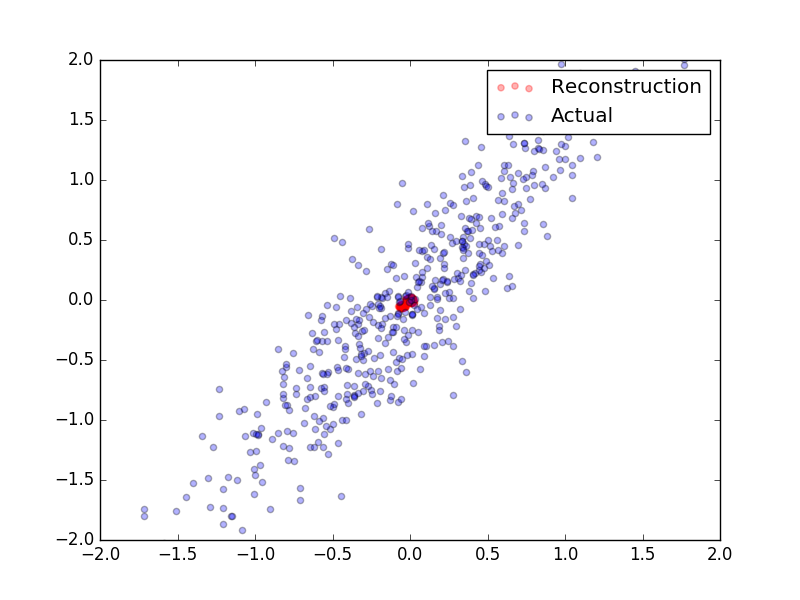
\includegraphics[width=0.68\columnwidth]{local_min_t}}
\caption{The MSE coverages but the weight matrix is trapped into a local minimum point and fails to come out.
(a): The evolution of the weights over iterations.
(b): The evolution of the mean square errors over iterations.
(c): The reconstructed $t_1-t_0$ and $t_2-t_0$.}
\label{local_minimum}
\end{figure*}

\begin{figure*}
\centering
\subfigure[$w_i$s]{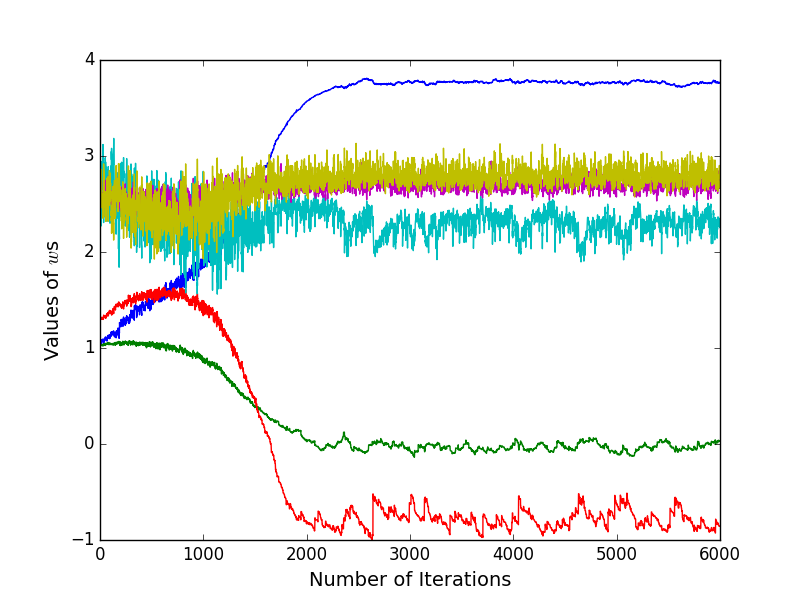
\includegraphics[width=0.68\columnwidth]{local_better_weight_evolution}}
\subfigure[MSE]{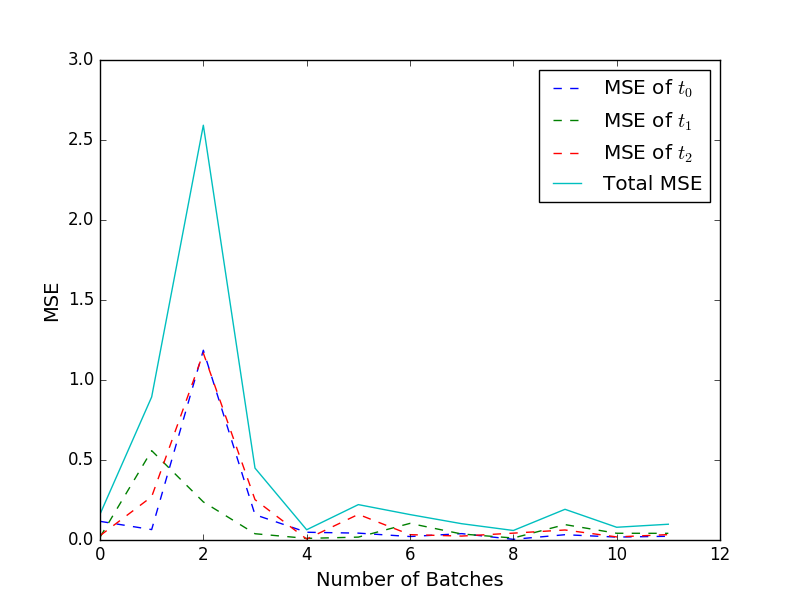
\includegraphics[width=0.68\columnwidth]{local_better_mse}}
\subfigure[Reconstructed $t_i$s]{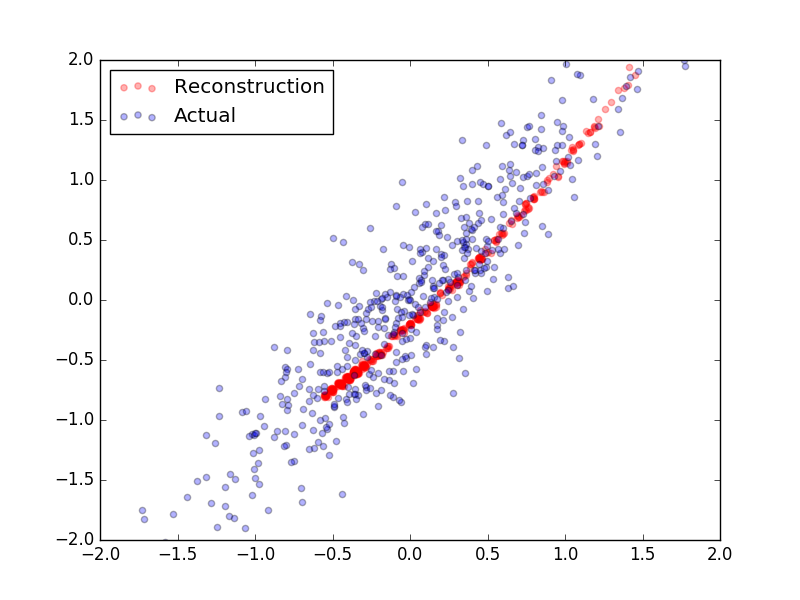
\includegraphics[width=0.68\columnwidth]{local_better_t}}
\caption{The weight matrix gets out of the local minimum point and converges to a better solution,
but it is trapped into another local minimum as
the reconstruction error is relatively large when $t_1 < t_0$ and $t_2 < t_0$.
(a): The evolution of the weights over iterations.
(b): The evolution of the mean square errors over iterations.
(c): The reconstructed $t_1-t_0$ and $t_2-t_0$.}
\label{local_better}
\end{figure*}

\begin{figure*}
\centering
\subfigure[$w_i$s]{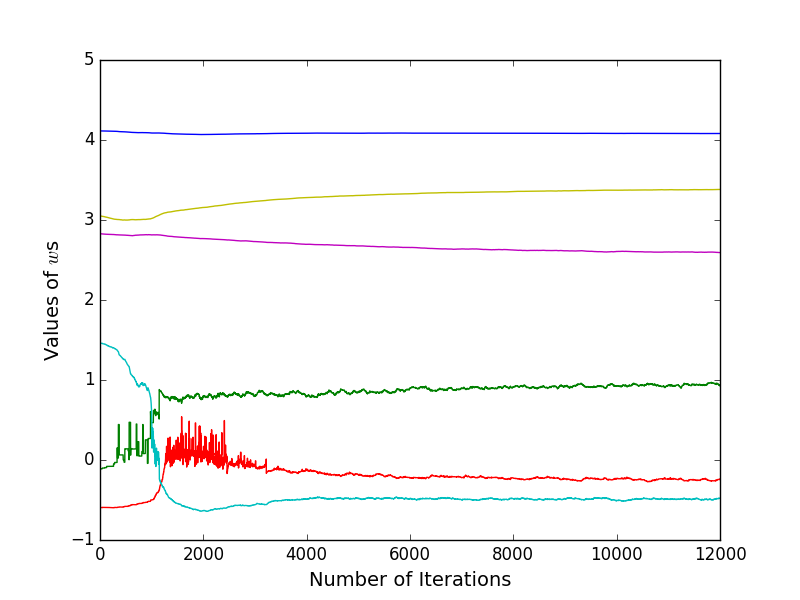
\includegraphics[width=0.68\columnwidth]{global_weight_evolution}}
\subfigure[MSE]{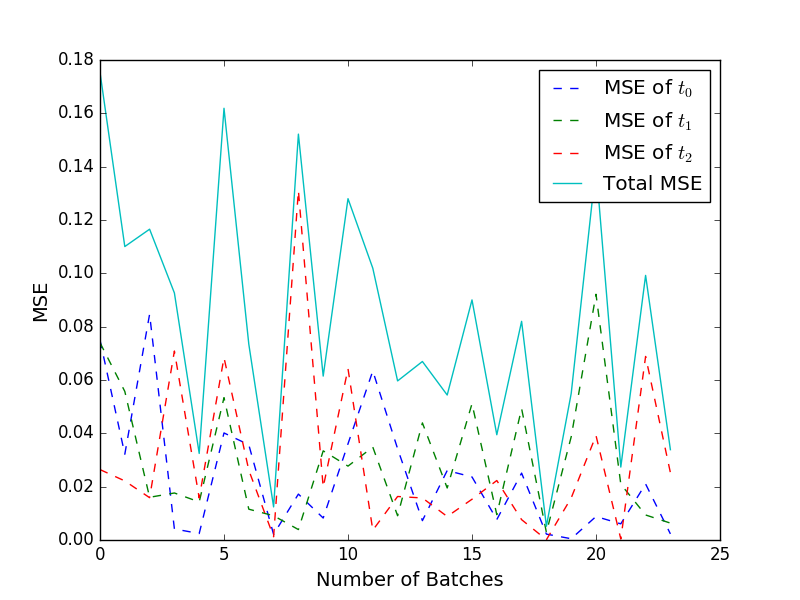
\includegraphics[width=0.68\columnwidth]{global_mse}}
\subfigure[Reconstructed $t_i$s]{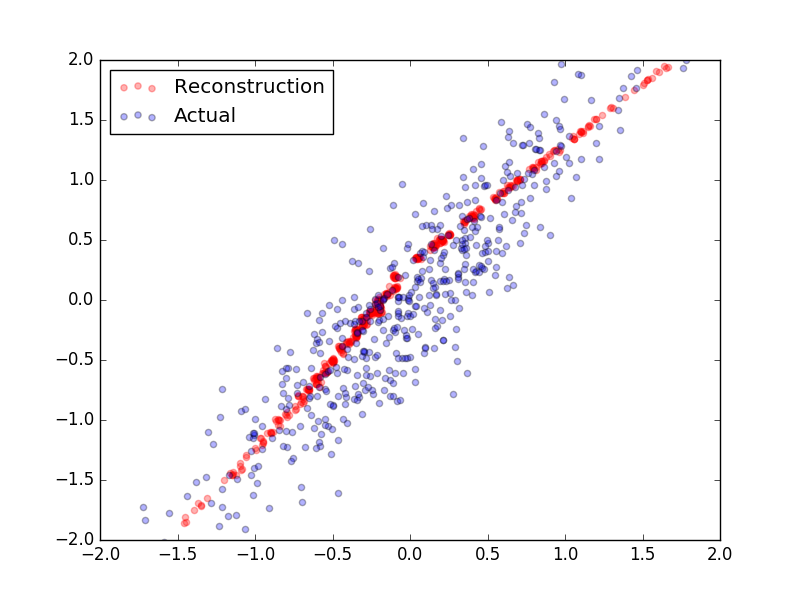
\includegraphics[width=0.68\columnwidth]{longer_better_t}}
\caption{Again the weight matrix gets out of the local minimum point and converges,
the total MSE further decreases, and the principal components are well reconstructed.
(a): The evolution of the weights over iterations.
(b): The evolution of the mean square errors over iterations.
(c): The reconstructed $t_1-t_0$ and $t_2-t_0$.}
\label{global_best}
\end{figure*}

\subsection{Encoding Natural Images}
Similarly, we continue working on the natural image encoding experiment mentioned in the paper. We use the same image dataset as the author's, which contains 10 gray images of size $512 \times 512$. We are supposed to randomly draw $16 \times 16$ patches from the gray images as our network input, normalizing all samples to scale their standard variation to 1. The encoder network has an architecture of $256\times 64 \times 256$, which means, the number of weight parameters to be trained in this network is over 10,000. Usually, we need a larger number of samples than weights to train a network model, however, with constraints of computation capacity, we only pick one $512 \times 512$ image, divide it to 1024 patches as the training data. To verify the correctness of the model, we reconstruct the same image with trained weights, to see whether a sparsely represented image could be obtained.

Unfortunately, we found tuning of parameters in this experiment is even harder than PCA. We adopt all parameters mentioned in paper, and adjust amplitude gain of Dirac current to be a reasonable value. Normalized to have a standard deviation of 1, the input value ranges from 0 to 4.8, which is a large range comparing to PCA case. The actual firing time can hardly fit the desired firing time, with weights updated every step by various samples.

We have tried different scales of learning rate $\eta$, as well as other parameters such like $C$, and $\lambda$. None of our trails results in a consistent convergence of MSE. We quite doubt on how the author tuned the parameter in such a non-convex problem, and how he avoid being trapped into local minima.

